% $HeadURL$

\subsection{Glyph: \glyph{State variable}}
\label{sec:stateVariable}

Biological entities can often exist under different states that affect
their function.  These ``states'' can arise for a variety of reasons.  For
example, macromolecules can be subject to post-synthesis modifications.  In
particular, residues of macromolecules (amino acids, nucleosides, or glucid
residues) can be modified by covalent linkage to other chemicals.  Another
example of states is alternative conformations, for instance, the closed,
open or desensitized conformations of a transmembrane channel, or the
active or inactive forms of an enzyme.  When an entity can exist under
different states, the state of the whole entity (the SBGN object) can be
described by the current values of all its state variables, and the values
of the state variables of all its possible components, recursively.

\begin{glyphDescription}

\glyphSboTerm Not applicable.

\glyphContainer A state variable is represented by an ellipsoid
  container, as shown in \fig{state-var}.  The ellipsoid's long axis should
  be tangent to the border of the glyph of the EPN being modified by the
  \glyph{state variable}.

  \glyphLabel The identification of an instance of a \glyph{state variable}
  is carried by one or two unbordered boxes, each containing a string of
  characters.  The characters cannot be distributed on several lines.  One
  box is mandatory, and contains the value of the \glyph{state variable}.
  The second box is optional and carries the identification of the
  \glyph{state variable}.  This identification should be present if
  confusion is possible between several state varibles (\eg several
  phosphorylation sites).  The center of the combination of the boxes
  located in the container box is superposed to the center of this
  container box.  Optionally, the identification of the \glyph{state
    variable} can be located outside the \glyph{state variable} container
  box.  This is \textbf{strongly} discouraged.  See \fig{wrong-state-var}
  below for some examples of problems arising if the identification of a
  state variable is located outside the state variable.

\glyphAux A \glyph{state variable} does not carry any auxiliary items.  

\end{glyphDescription}

\begin{figure}[H]
  \centering
  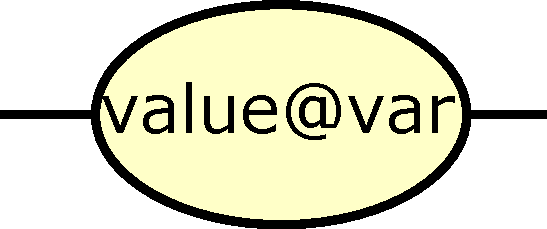
\includegraphics[scale = 0.3, trim = 0 0 0 0.25in]{images/stateVariable}
  \caption{The \PD glyph for \glyph{state variable}.}
  \label{fig:state-var}
\end{figure}

A \glyph{state variable} does not necessarily have to be a boolean-valued
variable.  For example, an ion channel can possess several conductance
states; a receptor can be inactive, active and desensitized; and so on.  A
\glyph{state variable} ``ubiquitin'' can also carry numerical values
corresponding to the number of ubiquitin molecules present in the tail.
However, a state variable can only take one defined value.  Furthermore, an
EPN's \glyph{state variable} should always be displayed and always set to a
value.  An ``empty'' \glyph{state variable} is a \glyph{state variable}
that is set to the value ``unset''.  Note that ``unset'' is \emph{not}
synonymous to ``any value'' or ``unknown value''.

The label of a state variable should, if possible, be displayed within the
ellipse.  In the top half of \fig{wrong-state-var} below, we show some
examples of pathological cases that lead to confusion in the association
between variable labels and values.  Compare the discouraged examples with
the recommended version in the bottom half of the figure.

\begin{figure}[H]
  \centering
  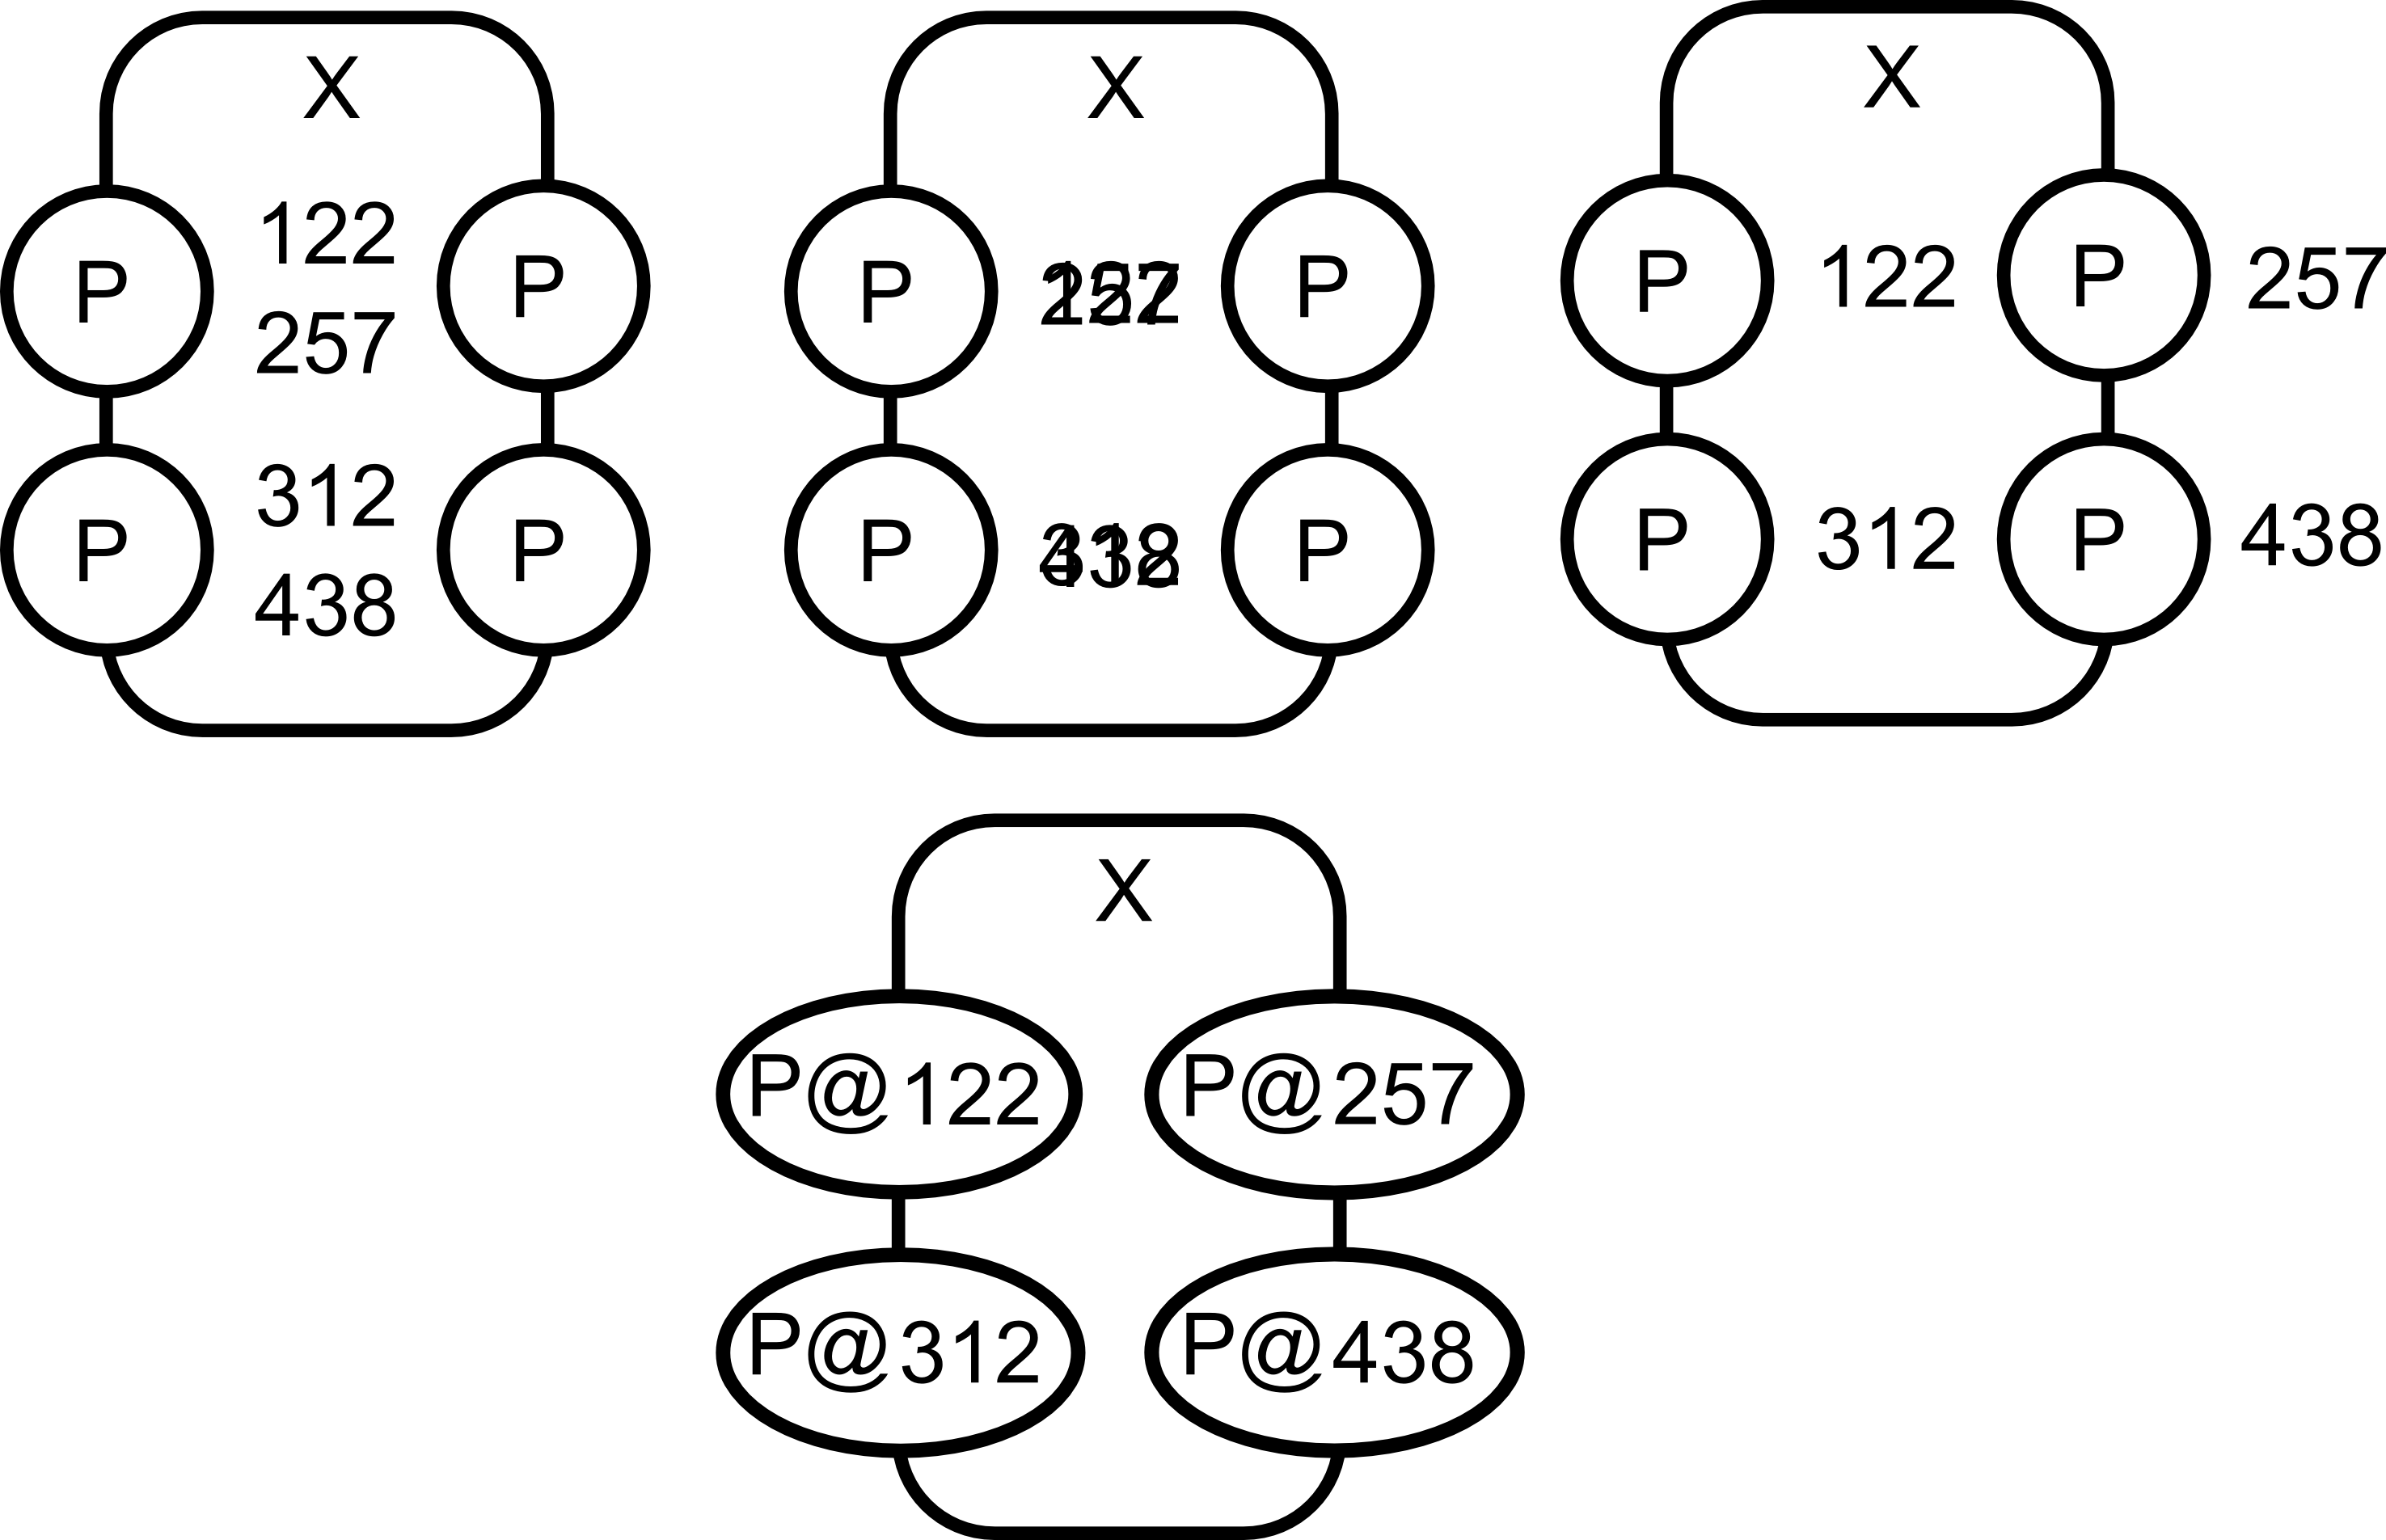
\includegraphics[scale = 0.3, trim = 0 0.5in 0 0.75in]{examples/wrongStateVariables}
  \caption{(Top) Examples of incorrect \glyph{state variables}.  (Bottom)
    Correct version.}
  \label{fig:wrong-state-var}
\end{figure}




% The following is for [X]Emacs users.  Please leave in place.
% Local Variables:
% TeX-master: "../sbgn_PD-level1"
% End:

